% !TEX encoding = UTF-8
% !TEX TS-program = pdflatex
% !TEX root = ../tesi.tex
% !TEX spellcheck = it-IT

%**************************************************************
\chapter{Funzionalità di disegno di elementi grafici 3D a scopo di debug}
\label{cap:game}
%**************************************************************

Lo studente è stato chiamato ad effettuare un refactor\footnote{Per effettuare refactor sono state seguite le linee guida spiegate in \cite{inbook:refactoring-book}.} ed implementare nuove funzionalità di disegno di oggetti 3D in game a scopo di debug. Le modifiche sono state apportate al gioco MotoGP 14, delle quali alcune sono state portate a MXGP HD.\\

Si è reso necessario dapprima un'analisi del codice allo scopo di individuare i flussi di interesse e localizzare le vecchie implementazioni su cui effettuare un refactor e sfruttare come base per l'implementazione delle nuove.\\

\section{Stampa dei livelli di LOD di moto e piloti}

In gioco esistono dei moduli grafici che implementano logiche di gestione degli actor di gioco. In particolare esistono in gioco due moduli che gestiscono il calcolo dei livelli di \gloss{LOD} per le moto ed i piloti. Entrambi i moduli sono istanze della classe \texttt{LodSelectionModule}\\

Gli algoritmi più utilizzati per calcolare i livelli di LOD degli oggetti in una scena 3D sono principalmente due. Il primo e più semplice è quello che calcola semplicemente la distanza fra la camera e l'oggetto 3D e scala i livelli secondo una generica funzione (la quale può cambiare a seconda delle tipologie di oggetti o particolari esigenze). Il secondo metodo invece consiste nel calcolare la quantità di pixel occupati dall'oggetto in relazione alla finestra di disegno. Essendo l'oggetto 3D potenzialmente formato da migliaia di poligoni, il calcolo preciso della superficie occupata richiederebbe molto più tempo di quello guadagnato scalando i livelli di dettaglio, si usa quindi un'approssimazione, ad esempio calcolando la superficie della bounding sphere.\\

Il secondo metodo risulta quasi necessario in giochi racing come MotoGP poiché esistono casi in cui il primo algoritmo fallisce molto più spesso del secondo. Si immagini ad esempio un grosso edificio in lontananza visibile dalla pista. Con il primo metodo, l'oggetto in questione, essendo distante, avrà il minimo livello di dettaglio disponibile anche se, essendo anche molto grande occuperà molto spazio su schermo, risultando sgradevole alla vista.\\

\begin{figure}[h!] 
	\centering 
	\hspace*{-0.05\columnwidth}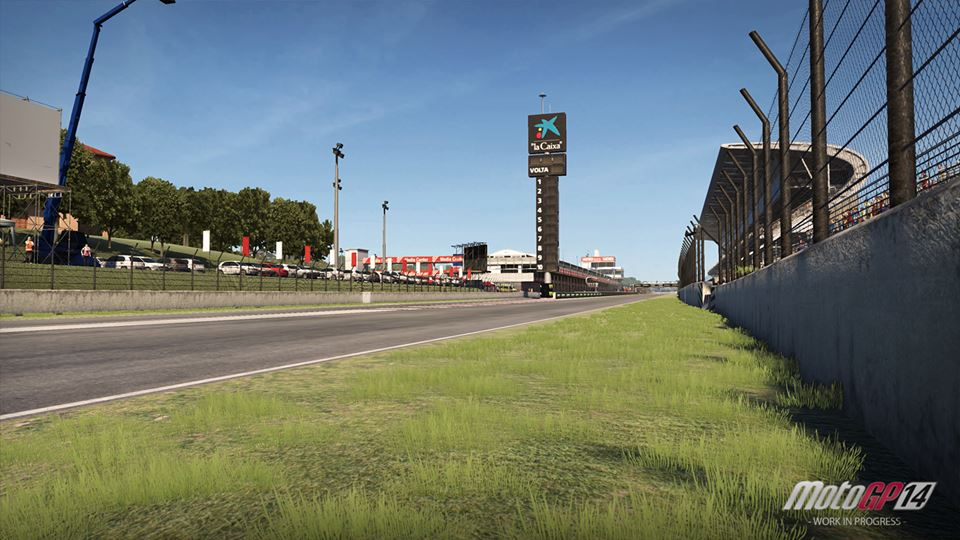
\includegraphics[width=1.1\columnwidth]{game/LODexample.jpg} 
	\caption{Screenshot di MotoGP 14: con il primo metodo la torre sarebbe al lod più basso, invece con il secondo continua ad essere gradevole alla vista}
\end{figure} 

Come già accennato in MotoGP 14 i moduli che gestiscono i livelli di LOD per moto e piloti sono due istanze della classe \texttt{LodSelectionModule}. Essa fornisce, attivabile da Beholder, la funzionalità di stampa dei livelli di LOD correnti degli oggetti per i quali gestisce il livello di dettaglio, in questo caso di moto e piloti presenti al momento in pista. Il problema in questo modulo, era la stampa dei livelli di LOD in posizioni errate, non permettendo di associare il LOD stampato con il suo oggetto. L'obbiettivo era quindi quello di avere la stampa dell'informazione affiancata all'oggetto, allo scopo di rendere più agevole e veloce il debug e il tuning per ogni piattaforma dell'algoritmo di scelta del LOD.\\

\begin{figure}[h!] 
	\centering 
	\hspace*{-0.05\columnwidth}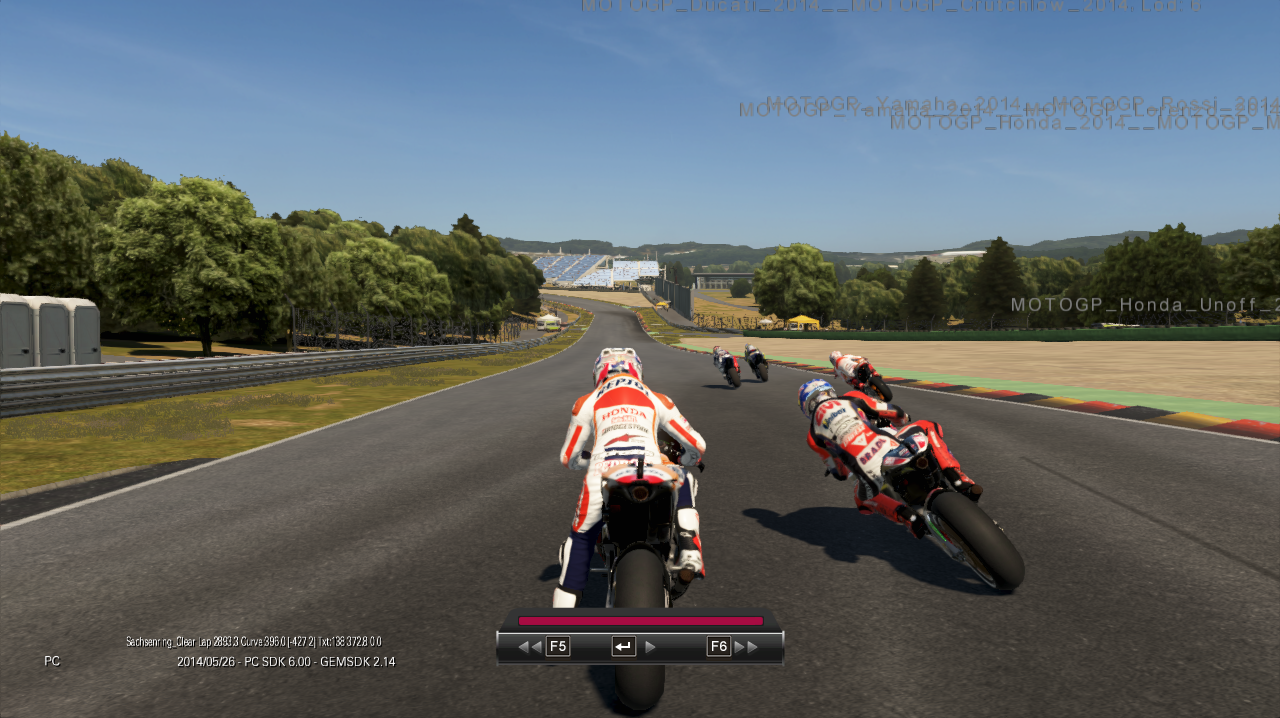
\includegraphics[width=1.1\columnwidth]{game/lodWritesBefore.png} 
	\caption{Screenshot di MotoGP 14 nel quale si può osservare la vecchia stampa dei livelli di LOD}
\end{figure}

Si parla di tuning dell'algoritmo per ciascuna piattaforma poiché, avendo caratteristiche hardware diverse, le varie piattaforme potranno gestire differenti combinazioni di oggetti con LOD alti. Esiste ad esempio un parametro che indica il massimo numero di bike con LOD 1\footnote{LOD 1 è il massimo livello di dettaglio.}. È compito del team 3D trovare i giusti parametri per permettere il miglior livello grafico possibile per ogni piattaforma.\\ 

Per risolvere il problema è stata inizialmente è stata quindi creata una funzione che trasformasse il punto 3D indicante la posizione dello scene actor, in un punto 2D relativo alle coordinate della finestra di gioco. Punto con il quale si procedeva con la stampa dell'informazione. Viene di seguito riportata la funzione creata.\\

\begin{lstlisting}[style=maurizio-code, caption=Metodo per la trasformazione di un punto 3D in un punto 2D della finestra di gioco rispetto la telecamera corrente, label={code:getScreenPosition}]
void GetScreenPosition(const CCamera* i_pCamera, GVector3& o_position) const
{	
	//Tranform to the homogeneous clip space
	
	//World transformation it's needed
	o_position.TransformPoint(poCamera->GetViewMatrix());
	o_position.TransformPoint(poCamera->GetProjMatrix());
	
	//Now the point is the range -1,1 for the x and y axis
	
	//Tranform to the windows space
	o_position.x = (o_position.x + 1) * poCamera->GetViewport().m_uiWidth;
	o_position.y = (o_position.y + 1) * poCamera->GetViewport().m_uiHeight;
	
	//The x cordinate of o_position is simply ignored 
}
\end{lstlisting}
~\\
La funzione \texttt{GetScreenPosition} procede a calcolare le stesse trasformazioni che esegue la GPU per trasformare ogni pixel dell'oggetto nella scena 3D in un'immagine 2D\footnote{Il lettore potrà trovare un approfondimento in \cite[chp.~5]{inbook:directx-book}.}. Si ottengono quindi le coordinate x e y dello schermo nello spazio -1, 1. Si procede quindi a trasformarle in coordinate relative allo spazio della finestra di gioco (ad esempio 1366x768 px).\\

Con un'analisi più approfondita del codice si è successivamente scoperto la presenza di un metodo della classe \texttt{CCamera} che produceva esattamente gli stessi risultati. Si è quindi provveduto a scartare questa implementazione (seppur corretta) ed usare quella già presente allo scopo di evitare inutili duplicazioni di codice.\\

Di seguito è presente la funzione della classe \texttt{LodSelectionModule} che lancia il disegno del LOD attivo. Questa funzione è lanciata per ogni oggetto gestito dalla classe.\\

\begin{lstlisting}[style=maurizio-code, caption=Metodo per la stampa del LOD corrente, label={code:printloddebuginformation}]
void LodSelectionModule::PrintLodDebugInformation(CWorld* iWorld, GraphicComponentInfo* i_pComponentInfo )
{
	//Foreach active camera
	for (GUInt camIdx = 0; camIdx < m_pWorld->GetNumberOfCameras(); ++camIdx)
	{
		//Get the string with the lod information and the name of the 3D object
		FixedString256 text;
		i_pComponentInfo->LodToString(camIdx, text);
		
		//Use the old function that calculates the screen point
		GVector2 screenPosition;
		iWorld->GetCurrentCamera(camIdx)->ProjectPoint(i_pComponentInfo->m_pBehavioutInput->GetMatrix().GetTranslation(), screenPosition);
		
		//Draw the LOD information
		DebugTextDrawer::GetInstance()->AppendLog(text.c_str(), screenPosition.x, screenPosition.y);
	}
}
\end{lstlisting}
~\\
Come si può facilmente capire dal codice l'invocazione del metodo \texttt{LodToString} compone la stringa che verrà stampata affianco all'oggetto 3D. Si è modificato tale metodo in modo tale che scrivesse come prima informazione il LOD e poi il nome dello scene actor. Questo perché se l'oggetto e nella parte destra della finestra e ha un nome lungo si corre il rischio che l'informazione più importante (il LOD) finisca fuori dal bordo e non sia visibile.

\begin{figure}[h!] 
	\centering 
	\hspace*{-0.05\columnwidth}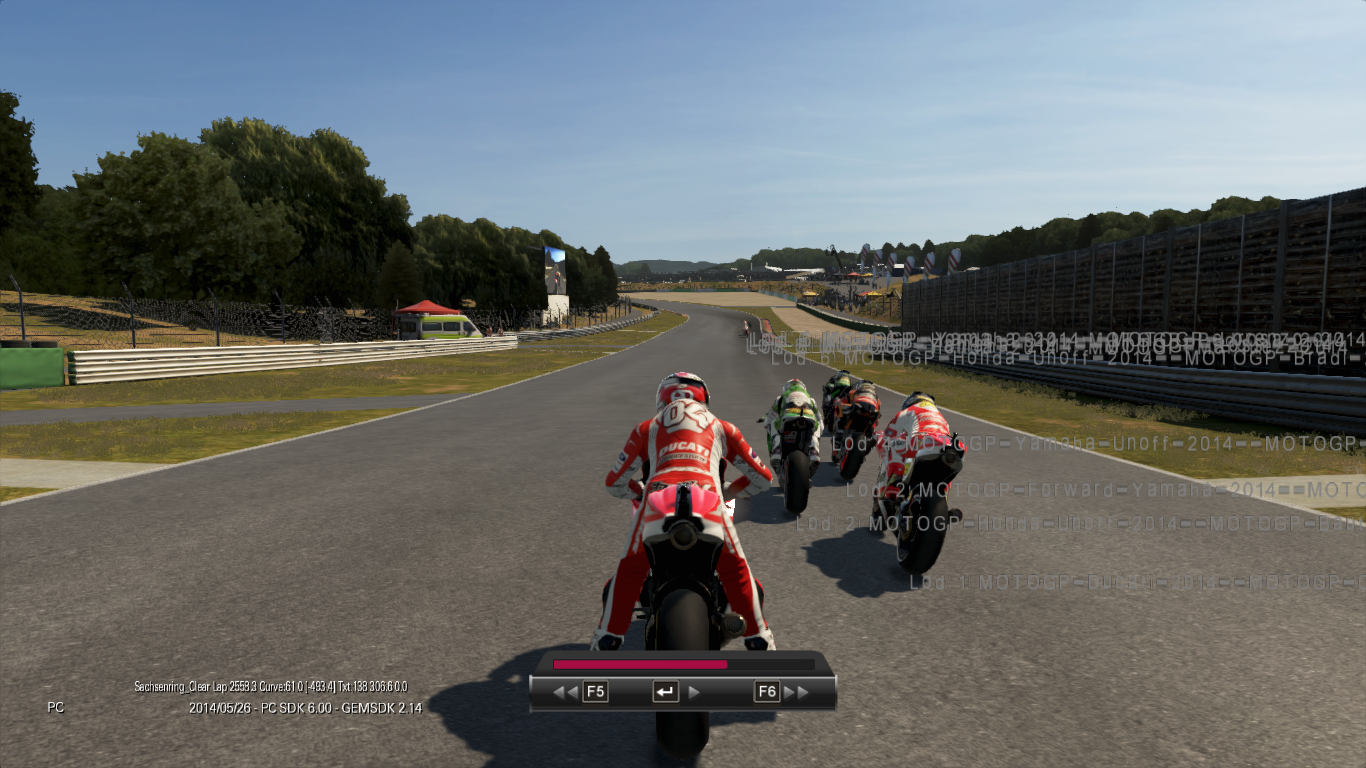
\includegraphics[width=1.1\columnwidth]{game/lodWritesAfterBike.png} 
	\caption{Screenshot di MotoGP 14 nel quale si può osservare la nuova stampa dei livelli di LOD per le moto}
\end{figure}

\begin{figure}[h!] 
	\centering 
	\hspace*{-0.05\columnwidth}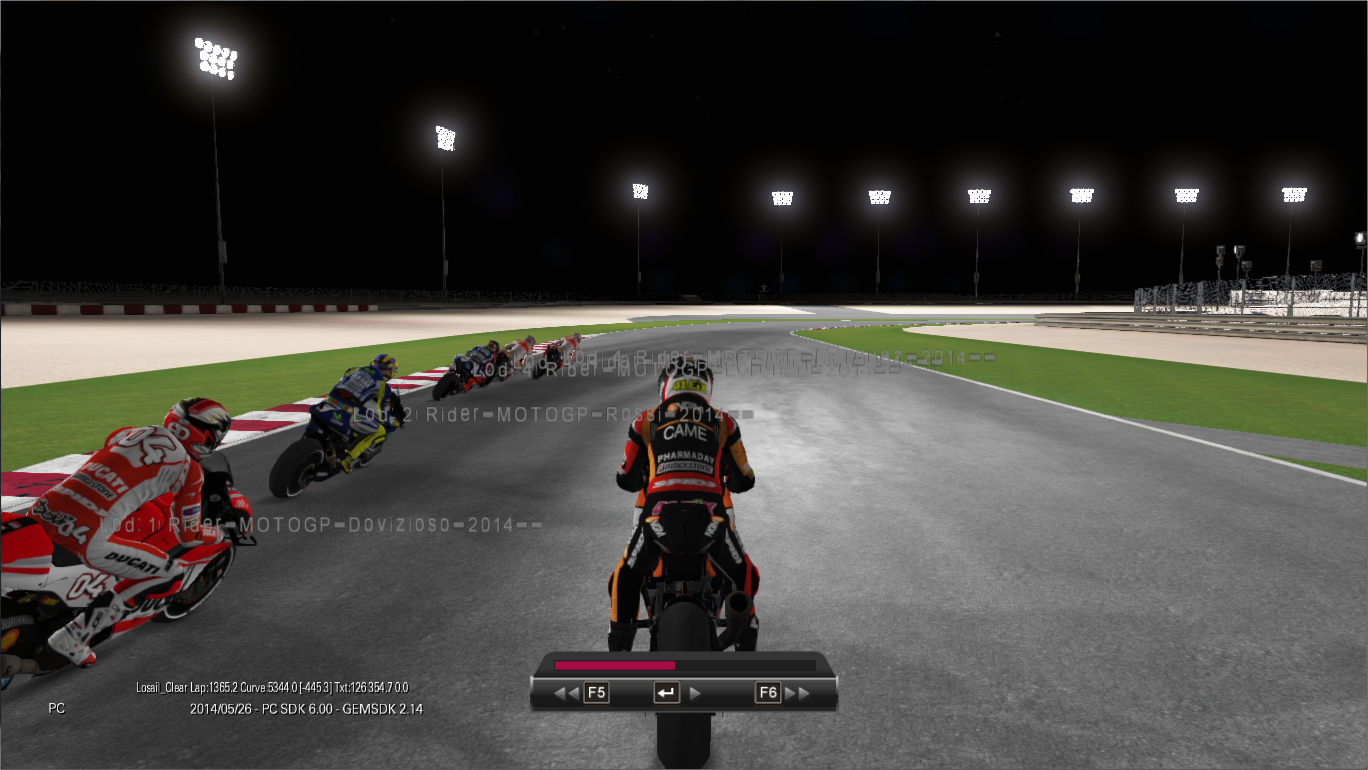
\includegraphics[width=1.1\columnwidth]{game/lodWritesAfterRider.png} 
	\caption{Screenshot di MotoGP 14 nel quale si può osservare la nuova stampa dei livelli di LOD per i piloti}
\end{figure}

Si è poi provveduto ad esporre nel Beholder una variabile membro per ogni istanza della classe \texttt{LodSelectionModule} che permette di attivare e disattivare la stampa di del LOD attivo a run-time.\\

\begin{figure}[h!] 
	\centering 
	\hspace*{-0.05\columnwidth}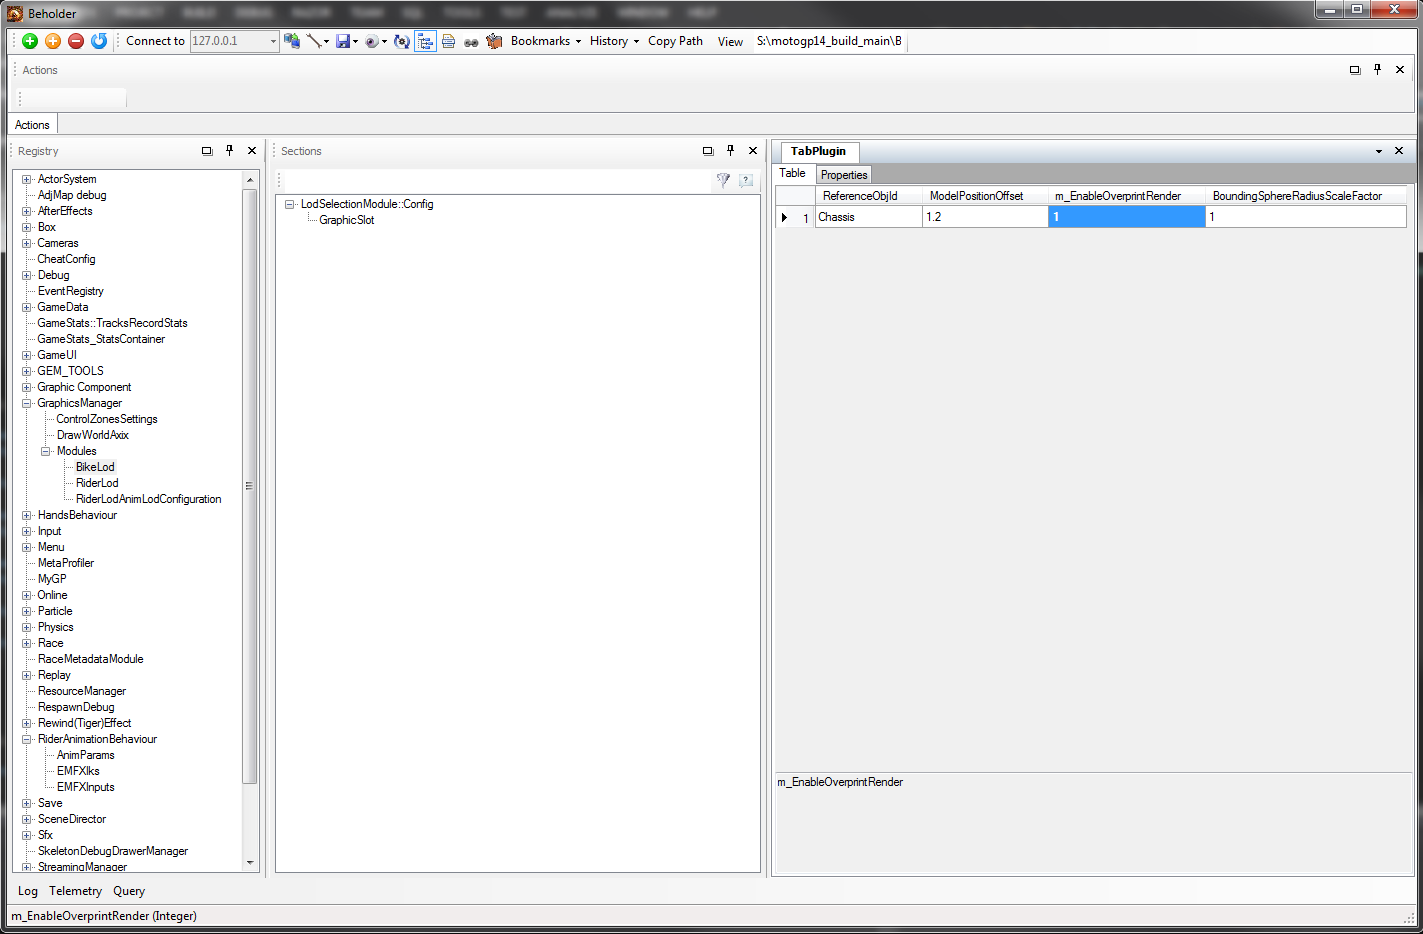
\includegraphics[width=1.1\columnwidth]{game/lodWritesBeholder.png} 
	\caption{Screenshot del Beholder nel quale è possibile vedere dove attivare e disattivare la stampa dei LOD delle moto}
\end{figure}

%\vspace{5cm}

\section{Rifattorizzazione della gerarchia di stampa}

Prestando attenzione al metodo \texttt{PrintLodDebugInformation} presente nel listato \ref{code:printloddebuginformation} si può notare che la stampa a video della stringa è affidata alla classe singleton \texttt{DebugTextDrawer}. Inizialmente la stampa era affidata in gestione alla classe \texttt{LodModuleDebug}, la quale aveva un nome completamente diverso dal compito che svolgeva. Indagando sulle origini di tale classe si è scoperto che questa era stata originata dal copia e incolla della classe \texttt{GemScreenLogger}, la quale gestiva la stampa di stringhe in stile terminale, conservando e ristampando le ultime entry inserite e gestendo gli \dq{a capo} e non permettendo sovrapposizioni del testo.\\

Avendo le due classi la maggior parte del codice in comune, si è provveduto ad effettuare un refactor creando una base astratta \texttt{UI\_GemScreenTextBase} dalla quale entrambe derivano e concretizzano implementando i metodi astratti. La classe \texttt{LodModuleDebug} è stata inoltre rinominata in \texttt{DebugTextDrawer} per meglio rispecchiare le sue funzionalità e rendere il codice più comprensibile.\\

\begin{figure}[h!] 
	\centering 
	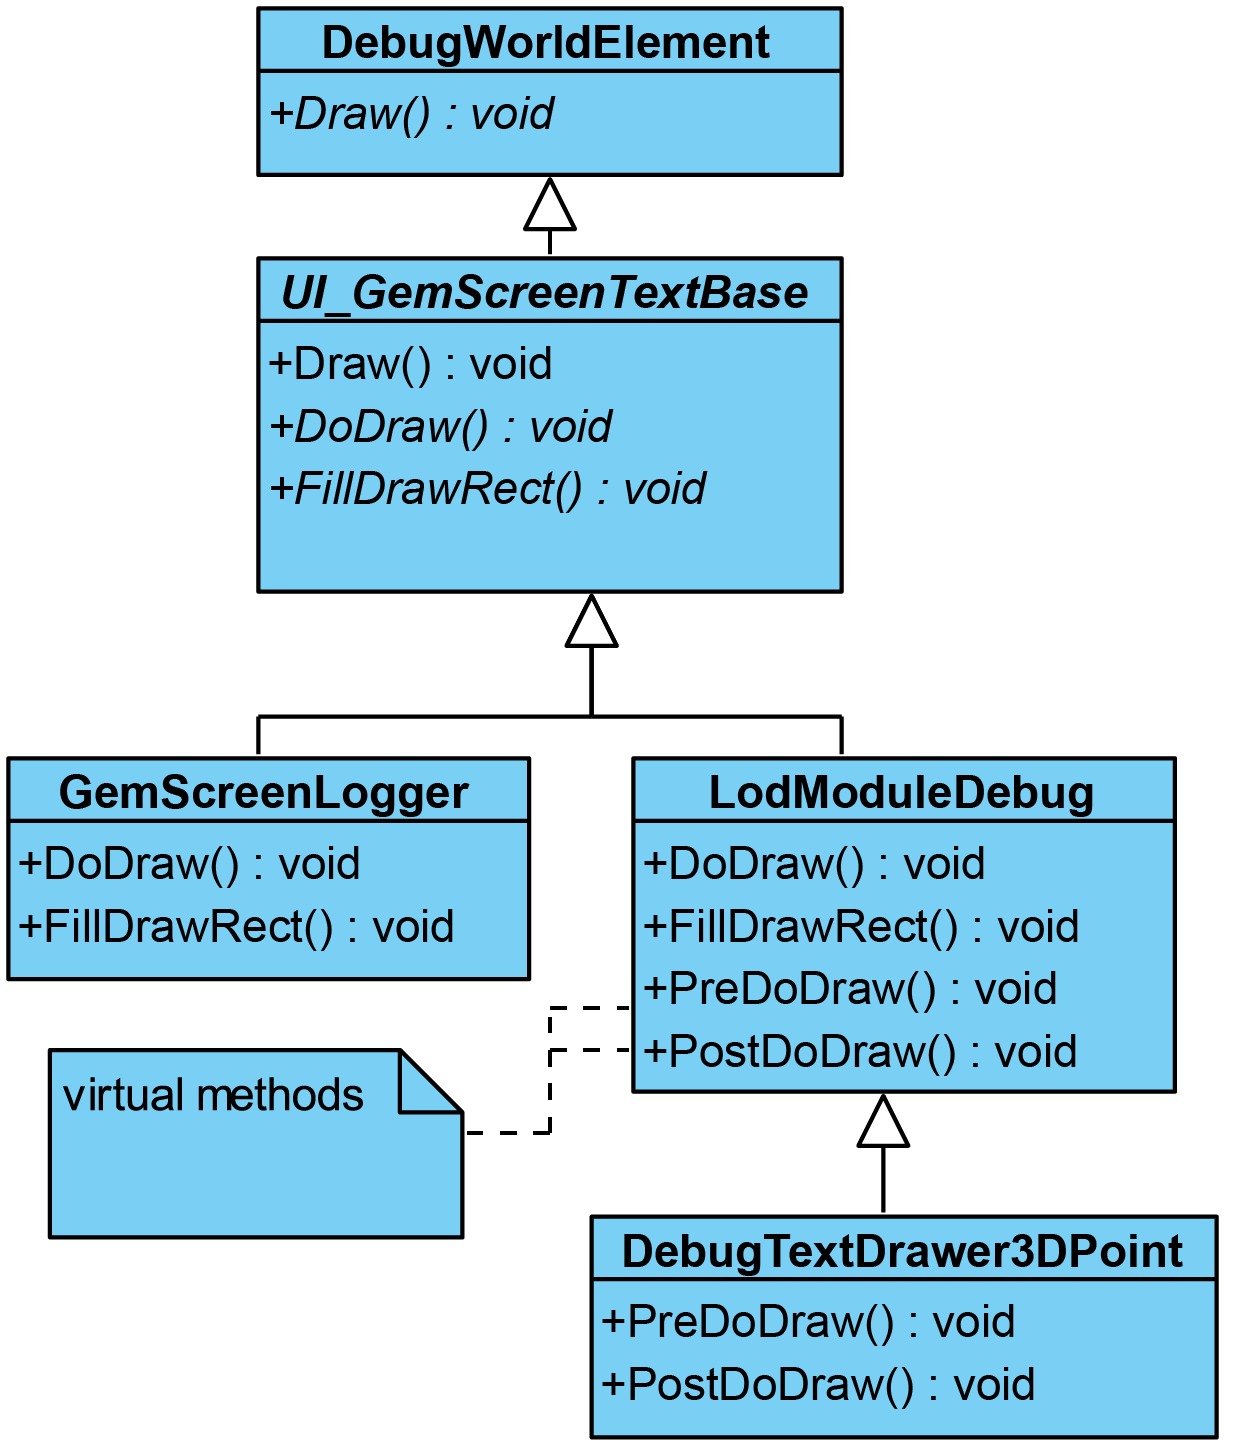
\includegraphics[width=0.6\columnwidth]{game/gerarchiaDrawText.png} 
	\caption{Diagramma UML della gerarchia di stampa del testo. Sono riportati solo i metodi più significativi}
\end{figure}

La classe \texttt{DebugTextDrawer3DPoint} verrà trattata successivamente nella sezione \ref{sec:stampa-del-nome-degli-spazi-di-riferimento}.\\

Le differenze fra le due classi si mostra anche nei loro scenari di utilizzo. \texttt{GemScreenLogger} accetta dei log e continua a stamparli indipendentemente dai frame. \texttt{DebugTextDrawer} invece, ad ogni frame, stampa tutte le stringhe che possiede e le scarta, non stampandole più al frame successivo. Questo impone quindi che l'inserimento delle scritte sia costante e presente ad ogni frame. Questa caratteristica si adatta perfettamente alla stampa dei LOD, in quanto la posizione su schermo e la stessa informazione varia ad ogni frame e necessita di un costante aggiornamento.\\ 

Come si nota dal diagramma (link diagramma) la gerarchia parte da \texttt{DebugWorldElement}, classe che rappresenta uno scene actor che può essere inserito in un world. I world sono dei contenitori di oggetti 3D che procedono, se attivi, ad ogni frame a disegnare ogni oggetto presente in essi.\\

Le istanze delle classi concrete della gerarchia vengono, durante la fasi di inizializzazione, inserite nel mondo di debug. Esso è stato creato appositamente per contenere oggetti di debug. Nel resto del gioco, sono presenti implementazioni più specifiche di world, le quali permettono quindi di fare assunzioni sugli oggetti presenti e conseguentemente implementare forti ottimizzazioni. In MotoGP 14 ad esempio sono presenti il \texttt{MenuWorld} ed il \texttt{GameWorld}, che gestiscono rispettivamente il mondo visibile nel menu di gioco ed il mondo visibile durante una gara, permettendone un disegno efficiente.\\

Di seguito è presente la sezione di codice che inizializza gli oggetti della gerarchia in fase di avvio del gioco:

\begin{lstlisting}[style=maurizio-code, caption=Inizializzazione delle classi responsabili della stampa di testo, label={code:initTextClasses}]
UI::GemScreenLogger::Create();
debugWorld->AddElement( UI::GemScreenLogger::GetInstance() );

GraphicModule::DebugTextDrawer::Create();
GraphicModule::DebugTextDrawer::Config config;
config.m_fontName = "Linotype Univers 430 Regular20"; //"ZZapDefaultFont"; alternativa funzionante
config.m_alphaValue = 255;
config.m_timeBeforeFade = 500;
config.m_includeContext = false;
config.m_includeSourceFile = false;
config.m_timestamp = false;
GraphicModule::DebugTextDrawer::GetInstance()->Init();
GraphicModule::DebugTextDrawer::GetInstance()->SetConfig( config );
debugWorld->AddElement( GraphicModule::DebugTextDrawer::GetInstance() );

GraphicModule::DebugTextDrawer3DPoint::Create();
GraphicModule::DebugTextDrawer3DPoint::GetInstance()->Init();
config.m_timeBeforeFade = 9999999999;
GraphicModule::DebugTextDrawer3DPoint::GetInstance()->SetConfig( config );
debugWorld->AddElement( GraphicModule::DebugTextDrawer3DPoint::GetInstance() );
\end{lstlisting}

\section{Stampa del nome degli spazi di riferimento}
\label{sec:stampa-del-nome-degli-spazi-di-riferimento}

Una funzionalità già presente è la stampa degli assi di riferimento degli oggetti presenti nella scena 3D e dell'asse origine del mondo. L'obbiettivo quindi è stato l'inserimento della stampa del nome dell'oggetto affianco al disegno dell'asse allo scopo di poterli riconoscere fra loro quando se ne disegnano più d'uno. Per realizzare questa funzionalità si è proceduto alla creazione della classe \texttt{DebugTextDrawer3DPoint}. Essa deriva da \texttt{DebugTextDrawer} della quale specializza semplicemente l'inserimento della stringa, allo scopo di poter continuare a disegnare il testo nella corretta posizione (che può cambiare) senza dover chiamare il disegno della stringa ogni frame. Il disegno degli assi è attivato dal Beholder da diversi contesti.\\

\begin{figure}[h!] 
	\centering 
	\hspace*{-0.05\columnwidth}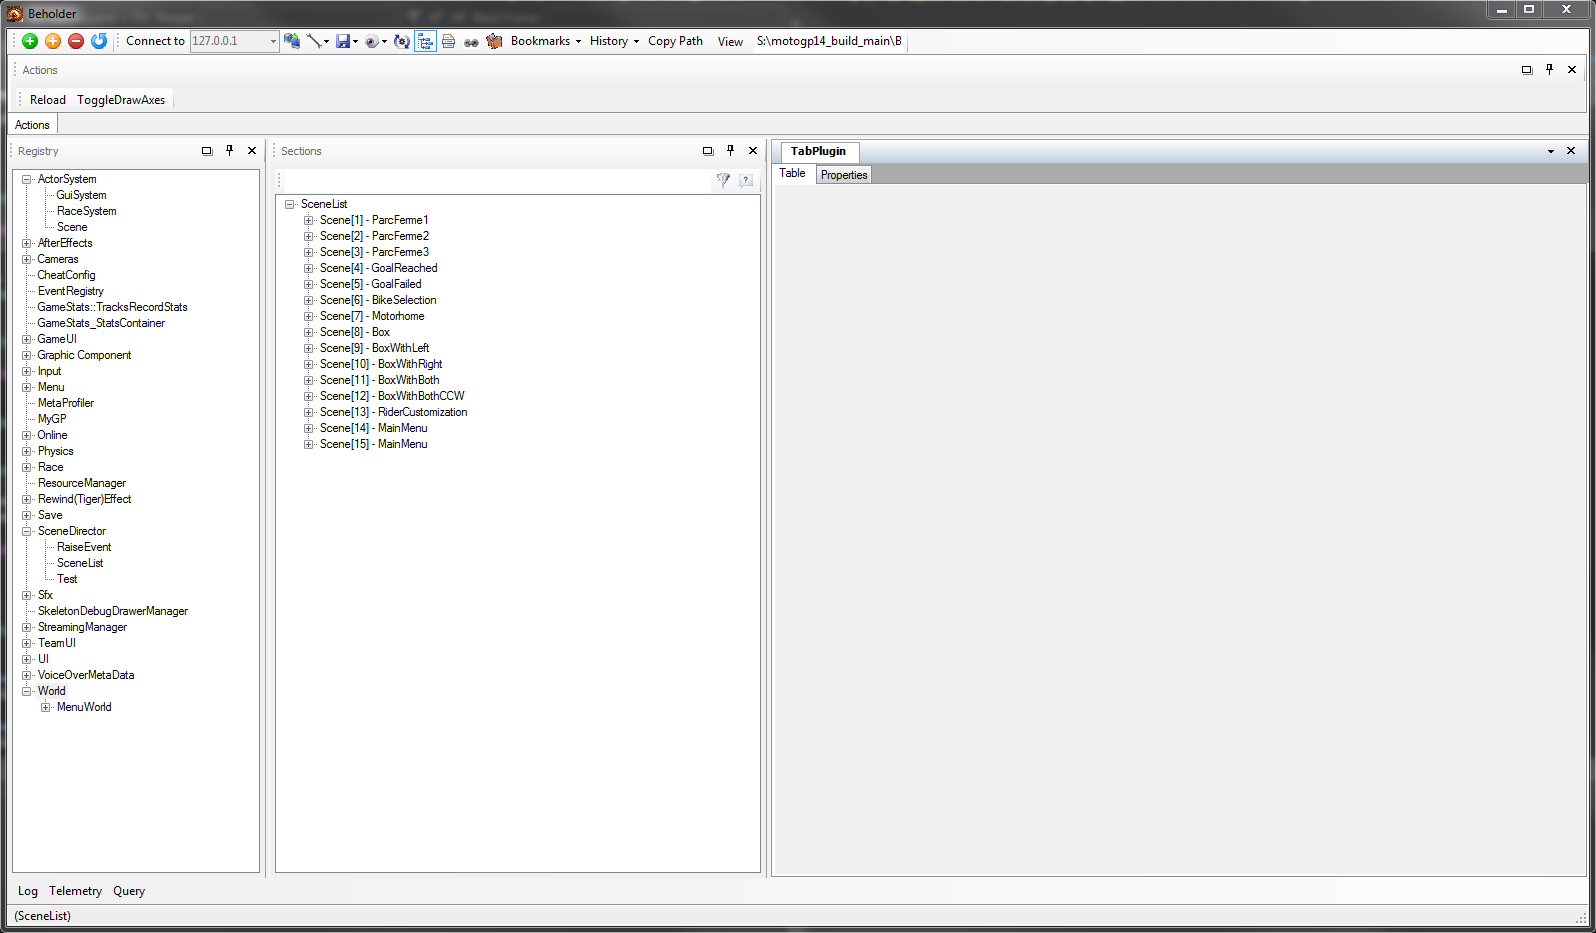
\includegraphics[width=1.1\columnwidth]{game/BeholderDrawSceneAxis.png} 
	\caption{Screenshot del Beholder nel quale è possibile lanciare il disegno degli assi tramite l'azione \dq{ToggleDraeAxes} dello \dq{SceneDirector} visibile in alto a sinistra}
\end{figure}

\texttt{DebugTextDrawer} provvede ad ogni frame, tramite un puntatore alla camera attiva e una reference alla matrice della posizione, che può quindi essere aggiornata, ad effettuare il calcolo del punto 3D a partire dal punto 2D e lanciare la stampa ad ogni frame. L'appesa di un log a questa classe richiede quindi della camera attiva, del testo e della matrice che contiene la posizione 3D. In questo modo è possibile disegnare il nome dell'asse, e continuare a visualizzare il nome ad ogni frame, senza dover appendere il log ad ogni frame come con \texttt{DebugTextDrawer}. Questo si è reso necessario in quanto il submit degli oggetti 3D che rappresentano gli assi avviene una volta soltanto, rendendo quindi necessaria l'utilizzo di un meccanismo simile anche per il testo correlato.

Lo studente ha provveduto quindi a individuare i punti del codice in cui erano presenti le chiamate di disegno degli assi allo scopo di implementare la nuova funzionalità, scoprendo che il codice per disegnarli era duplicato molteplici volte.\\

Si è proceduto quindi ad eseguire un refactor creando una classe specializzata nel disegno di assi con l'etichetta del nome dell'oggetto, la classe \texttt{DebugAxisDrawer}.\\

Essa provvede a incapsulare la funzione che si occupa del disegno degli assi e, eseguendo il codice necessario a ottenere la telecamera attiva, a lanciare lo stampa del nome dell'oggetto. Come accennato la funzionalità di disegno degli assi è lanciata durante un particolare stato in cui le geometrie disegnate, una volta eseguito il submit, vengono renderizzate ogni frame senza doverne richiederne la rappresentazione ad ogni frame. Si procede quindi allo stesso modo per il testo associato grazie alla classe \texttt{DebugTextDrawer3DPoint}.\\

Di seguito si riporta il codice della classe \texttt{DebugAxisDrawer}.

\lstinputlisting[style=maurizio-code, caption=DebugAxisDrawer.h, label={code:DebugAxisDrawer-h}]{code/DebugAxisDrawer.h}

\lstinputlisting[style=maurizio-code, caption=DebugAxisDrawer.cpp, label={code:DebugAxisDrawer-cpp}]{code/DebugAxisDrawer.cpp}

\begin{figure}[h!] 
	\centering 
	\hspace*{-0.05\columnwidth}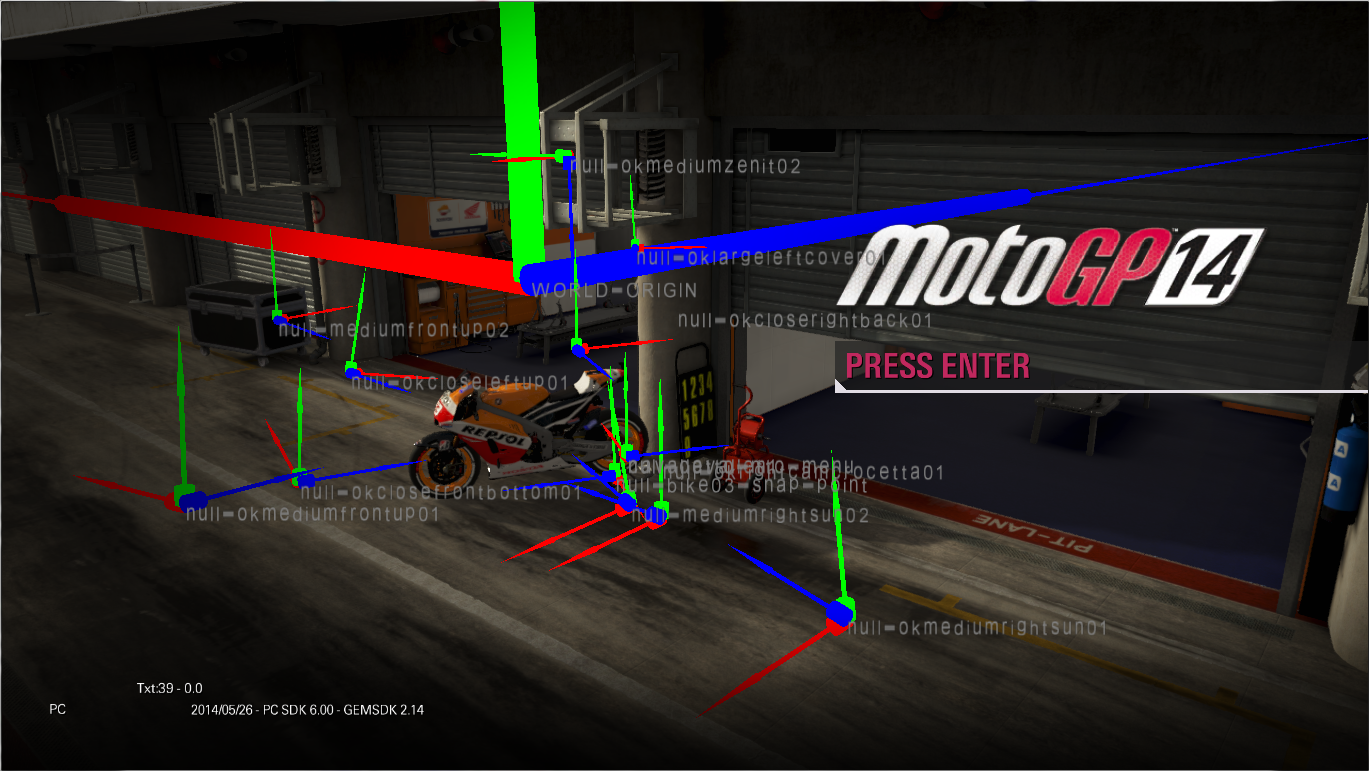
\includegraphics[width=1.1\columnwidth]{game/menuDrawAxisText.png} 
	\caption{Screenshot di MotoGP 14 in cui nel main menu è possibile vedere gli assi dei punti in cui viene ancorata la camera e la stampa del nome corrispondente}
\end{figure}

\section{Vista gerarchica dei world nel Beholder}
	Nel Beholder è possibile visualizzare tutte le risorse grafiche presenti nel \texttt{ResourcesManager}. Questa classe gestisce il caricamento e lo scaricamento in memoria di tutte le risorse grafiche utilizzate per costruire le scene 3D del gioco. Essa utilizza la strategia di reference couting per sapere quando un oggetto diviene inutilizzato e può essere quindi scaricato. Essa contiene quindi una collezione di world in cui sono presenti le varie risorse (mesh, texture, animazioni, ecc..). Per ogni tipo di risorsa presente nel word nel Beholder viene presentata come lista piatta. È possibile invece che queste risorse siano imparentate fra di loro, formando ad esempio delle gerarchie di oggetti 3D.\\
	
	\begin{figure}[h!] 
		\centering 
		\hspace*{-0.05\columnwidth}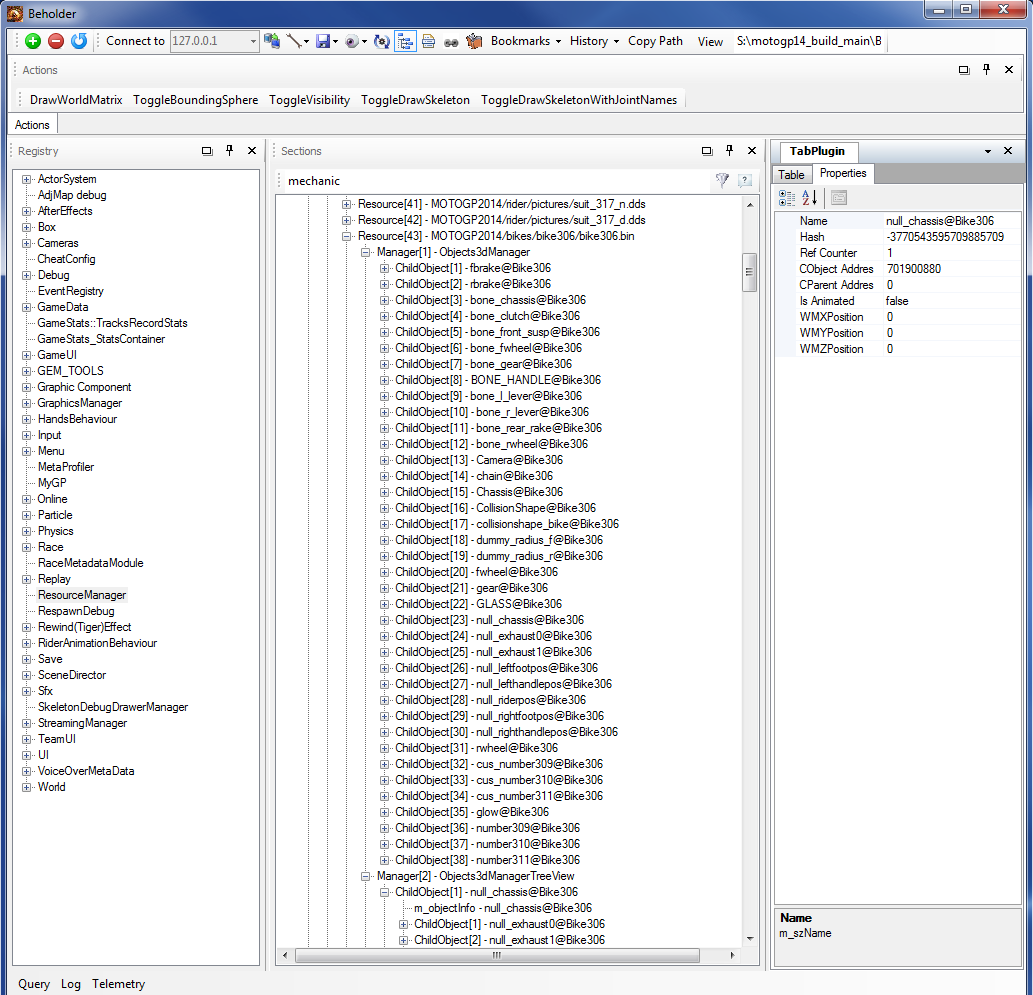
\includegraphics[width=1.1\columnwidth]{game/beholderResourceManagerView.png} 
		\caption{Screenshot del Beholder in cui è possibile visualizzare la versione a lista piatta sopra e la versione ad albero sotto per la bike 306}
		\label{fig:resource-manager-tree-view}
	\end{figure}
	
	Si è proceduto quindi a creare una versione ad albero per la categoria degli Object3D presenti nel world.\\
	
	Il contenuto del \texttt{ResourcesManager} è esposto nel Beholder tramite la classe \texttt{ResourcesManagerDebug} in cui si concentrano le modifiche effettuate per poter offrire la nuova funzionalità.
	
	Di seguito vengono riportati alcune sezioni del codice della classe significative per la nuova funzionalità inserita.
	
	\lstinputlisting[style=maurizio-code, caption=ResourcesManagerDebug.h, label={code:ResourcesManagerDebug-h}]{code/ResourcesManagerDebug_new.h}
	
	\lstinputlisting[style=maurizio-code, caption=ResourcesManagerDebug.cpp, label={code:ResourcesManagerDebug-cpp}]{code/ResourcesManagerDebug_new.cpp}
	
	\lstinputlisting[style=maurizio-code, caption=ResourcesManagerDebug\_Metadata.cpp, label={code:ResourcesManagerDebug-Metadata-cpp}]{code/ResourcesManagerDebug_newMetadata.cpp}

\section{Disegno degli scheletri di animazione}
	
	Allo scopo di permettere agli artisti di affinare le animazioni scheletrali dei personaggi e permettere al team 3D un più rapido debug, è stato deciso di aggiungere al gioco la funzionalità di disegno dello scheletro di animazione degli oggetti animati.\\
	
	Come visibile in figura \ref{fig:SkeletonTerminology} lo scheletro di animazione è composto da un'insieme di bone (ossa) organizzati gerarchicamente: se il padre viene mosso, il movimento e trasmesso a tutta la prole. Un modo efficiente di memorizzare lo scheletro è tramite una palette di matrici \footnote{Nella grafica 3D una matrice 4x4 è un modo efficiente di memorizzare una posizione oppure una trasformazione in termini di traslazione, rotazione e scale. Un approfondimento è disponibile in \cite[chp.~3]{inbook:directx-book}} che rappresentano la posizione dei joint (estremi esterni di un bone) che compongono lo scheletro. È inoltre necessaria una lista che permetta di sapere come è organizzata la gerarchia dei joint per permettere la ricostruzione dello scheletro\footnote{Esistono metodi di memorizzazione più efficienti utilizzando strutture dati avanzate ma, visto che solitamente lo scheletro viene sempre scorso linearmente e i bone vengono raramente rimossi o aggiunti, questa è una delle implementazioni più usate nella computer grafica.}.\\
	
	\begin{figure}[h!] 
		\centering
		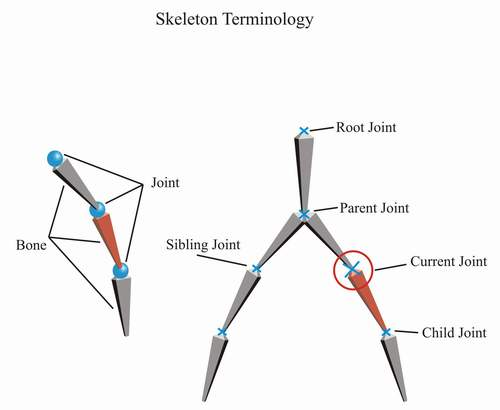
\includegraphics[width=0.8\columnwidth]{game/SkeletonTerminology.jpg}
		\caption{Una sintesi della terminologia appena introdotta. Tratto da \cite{site:skeleton-terminoligy}}
		\label{fig:SkeletonTerminology}
	\end{figure}
	
	
	Si procede quindi ad animare\footnote{Si consiglia al lettore appassionato \cite[chp.~24, 25]{inbook:directx-book} in cui è presente una breve introduzione alla matematica dei quaternioni, l'animazione scheletrale e lo skinning.} lo scheletro di animazione tramite la fisica o con delle pose fisse precalcolate dagli artisti, oppure con il blend tree calcolato tramite il middleware Emotion Fx.\\
	
	Il passo successivo è modificare la mesh dell'oggetto per rispecchiare l'animazione dello skeleton, questa procedura è detta Skinning. Un modo semplice per effettuarla è assegnare ad ogni vertice della mesh un massimo di 4 bone che potranno influenzarne la posizione. Si procede quindi (solitamente su GPU durante la fase di Vertex Shader) a calcolare un'interpolazione sulla trasformazione della posizione del vertice effettuando una media pesata fra i bone assegnati. La trasformazione risultante viene quindi applicata alla posizione originale del vertice.\\
	
	L'analisi del codice di gioco ha evidenziato la presenza di una precedente implementazione del disegno dello skeleton dei soli rider durante la corsa. Questa implementazione permetteva l'attivazione e la disattivazione della funzionalità di disegno attraverso una \texttt{define}.\\

	La prima modifica è stata l'esposizione nel Beholder di una variabile di membro di quella classe che permettesse di attivare/disattivare il disegno di debug a run-time.\\
	
	\begin{figure}[h!] 
		\centering 
		\hspace*{-0.05\columnwidth}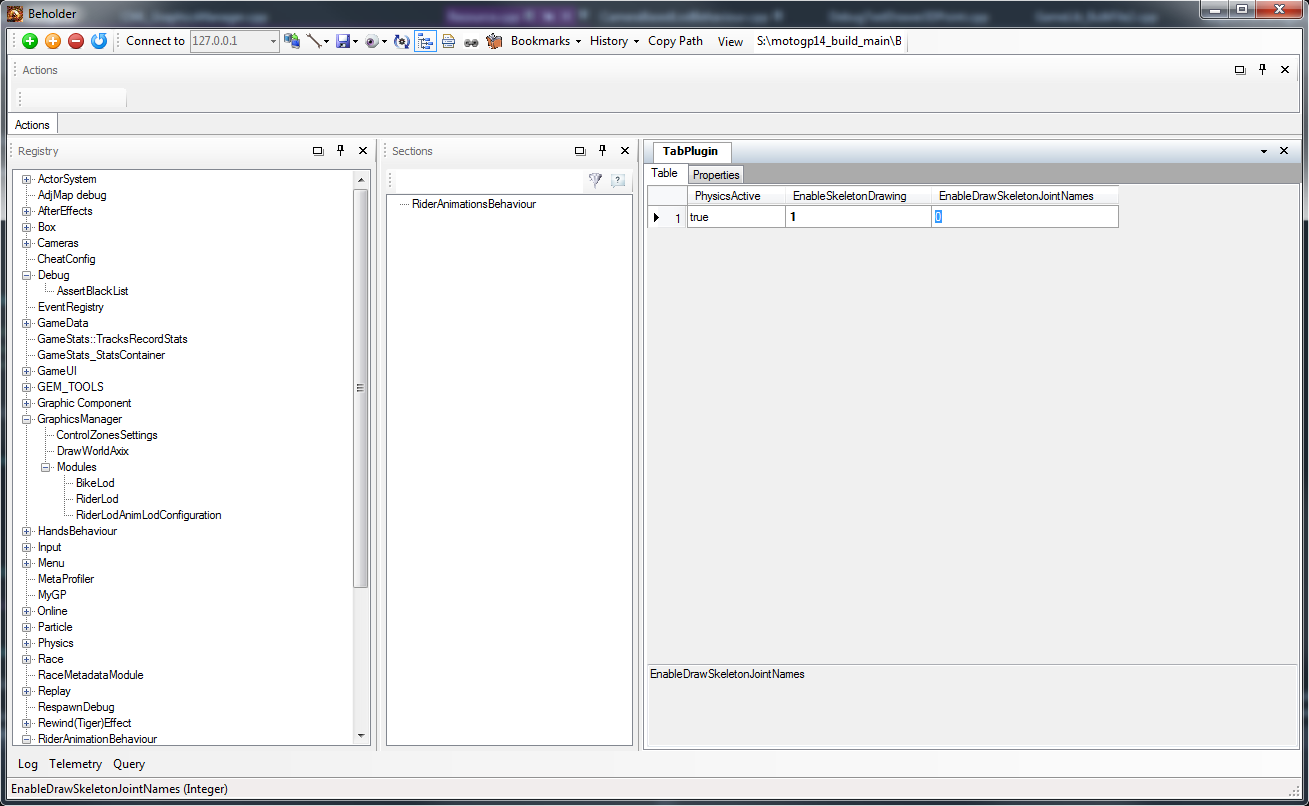
\includegraphics[width=1.1\columnwidth]{game/BeholderActivateRiderSkeleton.png} 
		\caption{Screenshot del Beholder in cui è possibile visualizzare dove è permesso attivare e disattivare il disegno dello skeleton del rider}
	\end{figure}
	
	Successivamente si è proceduto ad affinare e ottimizzare l'algoritmo di disegno, estrapolandolo e portandolo in una classe specializzata nel solo disegno di uno skeleton: \texttt{SkeletonDebugDrawer}.\\
	
	Di seguito è presente il codice della classe \texttt{SkeletonDebugDrawer}.
	
	\lstinputlisting[style=maurizio-code, caption=SkeletonDebugDrawer.h, label={code:SkeletonDebugDrawer-h}]{code/SkeletonDebugDrawer.h}
	
	\lstinputlisting[style=maurizio-code, caption=SkeletonDebugDrawer.cpp, label={code:SkeletonDebugDrawer-cpp}]{code/SkeletonDebugDrawer.cpp}
	~\\
	La rappresentazione interna dello scheletro organizzata come spiegato prima, permette quindi di utilizzare lo scheletro efficientemente minimizzando le moltiplicazioni tra matrici. L'algoritmo di disegno procede quindi ricorsivamente, con un approccio top-down, a calcolare l'effettiva posizione del joint corrente applicando la trasformazione del padre. In questo modo si evitano la ripetizione della stessa operazione che sarebbe emersa in un approccio bottom-up.\\
	
	\begin{figure}[h!] 
		\centering 
		\hspace*{-0.05\columnwidth}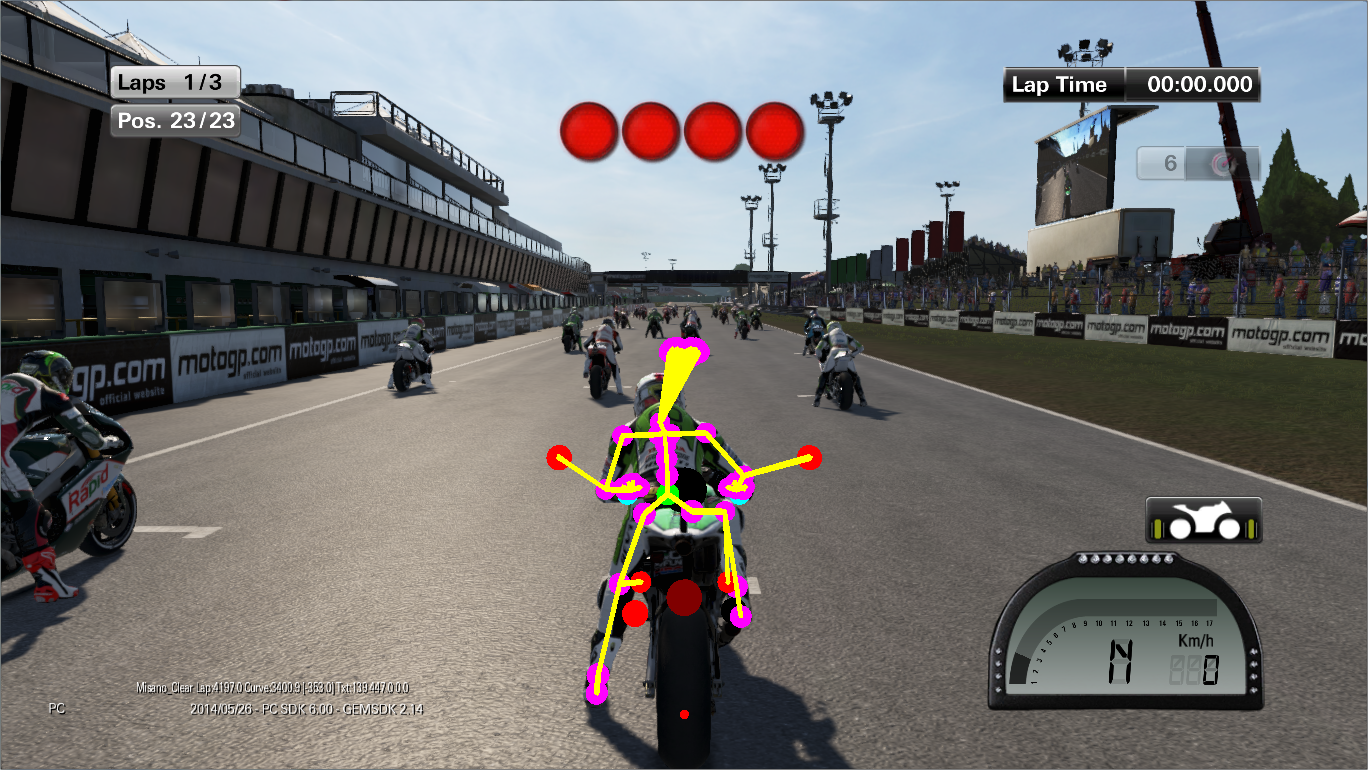
\includegraphics[width=1.1\columnwidth]{game/skeletonRider1.png} 
		\caption{Screenshot n. 1 del disegno dello skeleton del rider}
	\end{figure}
	
	\begin{figure}[h!] 
		\centering 
		\hspace*{-0.05\columnwidth}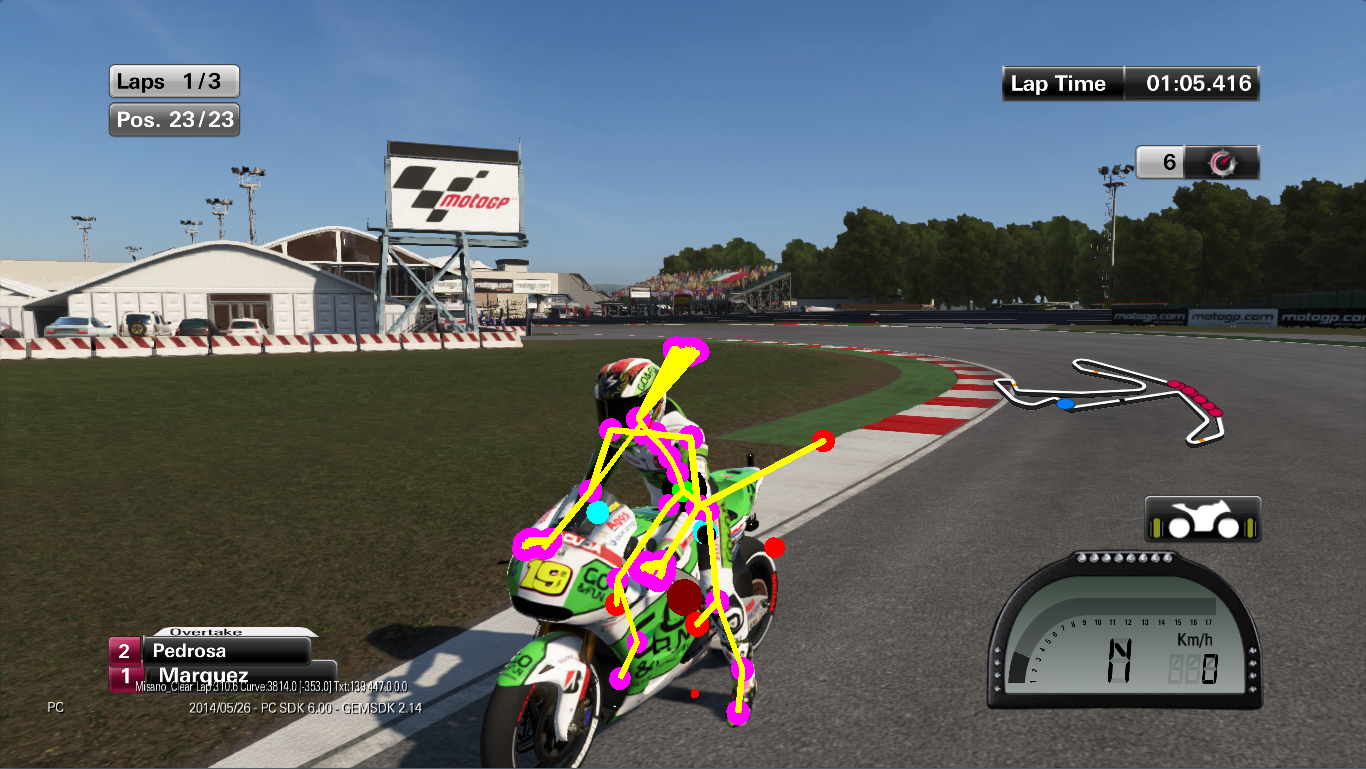
\includegraphics[width=1.1\columnwidth]{game/skeletonRider2.png} 
		\caption{Screenshot n. 2 del disegno dello skeleton del rider}
	\end{figure}
	
	Un altro obbiettivo era quello di disegnare lo scheletro di animazione non solo del rider corrente ma, di un qualsiasi oggetto animato.\\
	
	Per soddisfare questo obbiettivo si è ricorsi al \texttt{ResourcesManagerDebug}. Esso contenendo tutti gli oggetti era il posto corretto da cui partire. Per ogni \texttt{CObject3d} si è proceduto a valutare se era un oggetto animato e nel caso, permettere all'utente tramite Beholder di lanciare il disegno dello scheletro.\\
	
	Per capire se un oggetto è animato si è ricorsi ad un dynamic\_cast da \texttt{CObject3d} a \texttt{CAnimated3dModel}, sottoclasse che rappresenta gli oggetti 3d anche animati. Nel codice il dynamic\_cast è stato poi sostituito con un più veloce confronto tra ClassID.\\
	
	Per gli oggetti animati è stato quindi inserito nel Beholder la possibilità di lanciarne il disegno dello scheletro. Essendo il disegno dello scheletro un'azione da compiere ad ogni frame, vista la sua continua modifica, si è proceduto a creare la classe \texttt{SkeletonDebugDrawerManager}. Essa permette di aggiungere un oggetto il cui scheletro verrà disegnato ogni frame. Permette inoltre di mettere in pausa il disegno oppure di fermare definitivamente il disegno.\\
	
	Come già accennato tutte queste funzionalità sono disponibili da Beholder, in particolare per ogni oggetto visualizzato nel Beholder tramite il \texttt{ResourcesManagerDebug} è presente una proprietà che indica (true o false) se l'oggetto è animato, e quindi è possibile disegnarne lo scheletro.\\
	
	In figura \ref{fig:resource-manager-tree-view} è visibile sulla destra le proprietà di un oggetto 3D, tra le quali \texttt{isAnimated}. In alto a sinistra invece ci sono le azioni disponibili, tra le quali il disegno dello scheletro. Azione che verrà davvero eseguita solo se l'oggetto è animato.
	
	\begin{figure}[h!] 
		\centering 
		\hspace*{-0.05\columnwidth}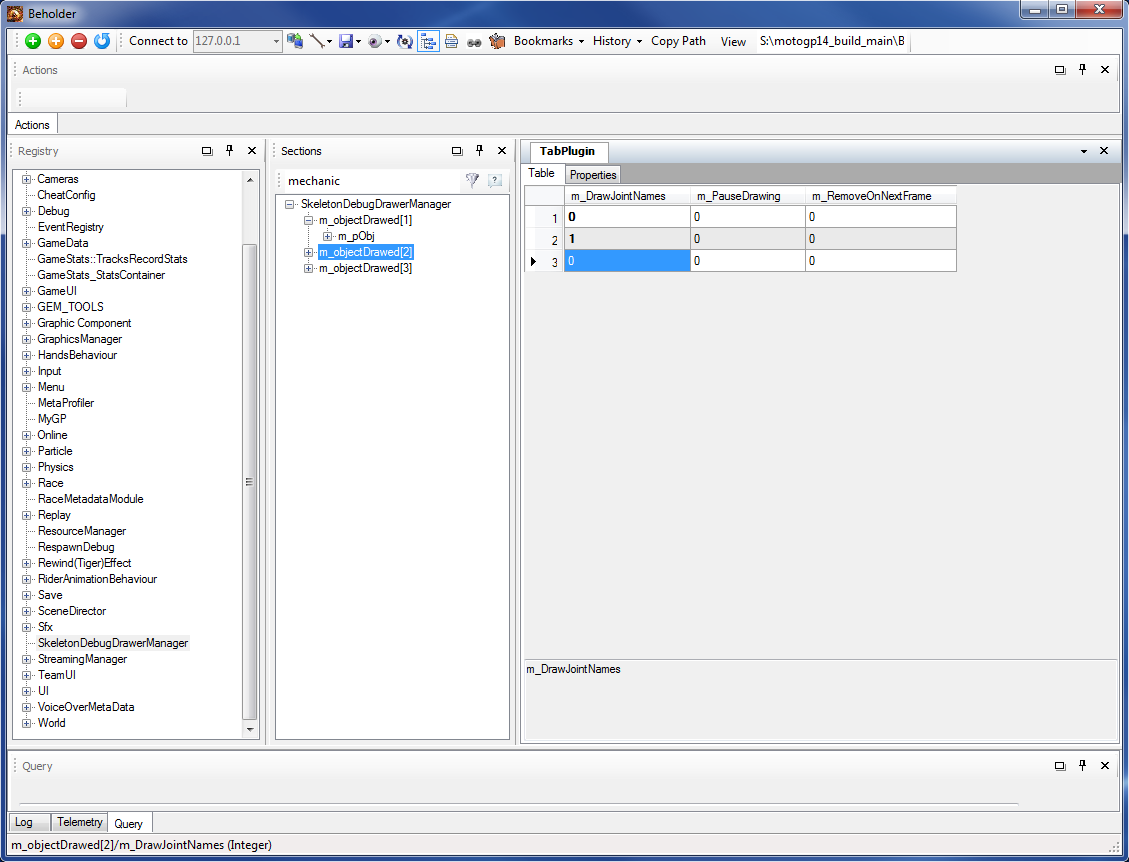
\includegraphics[width=1.1\columnwidth]{game/SkeletonDebugDrawerManagerinBeholder.png} 
		\caption{Screenshot del Beholder in cui è visibile lo \texttt{SkeletonDebugDrawerManager}}
	\end{figure}
	
	\begin{figure}[h!] 
		\centering 
		\hspace*{-0.05\columnwidth}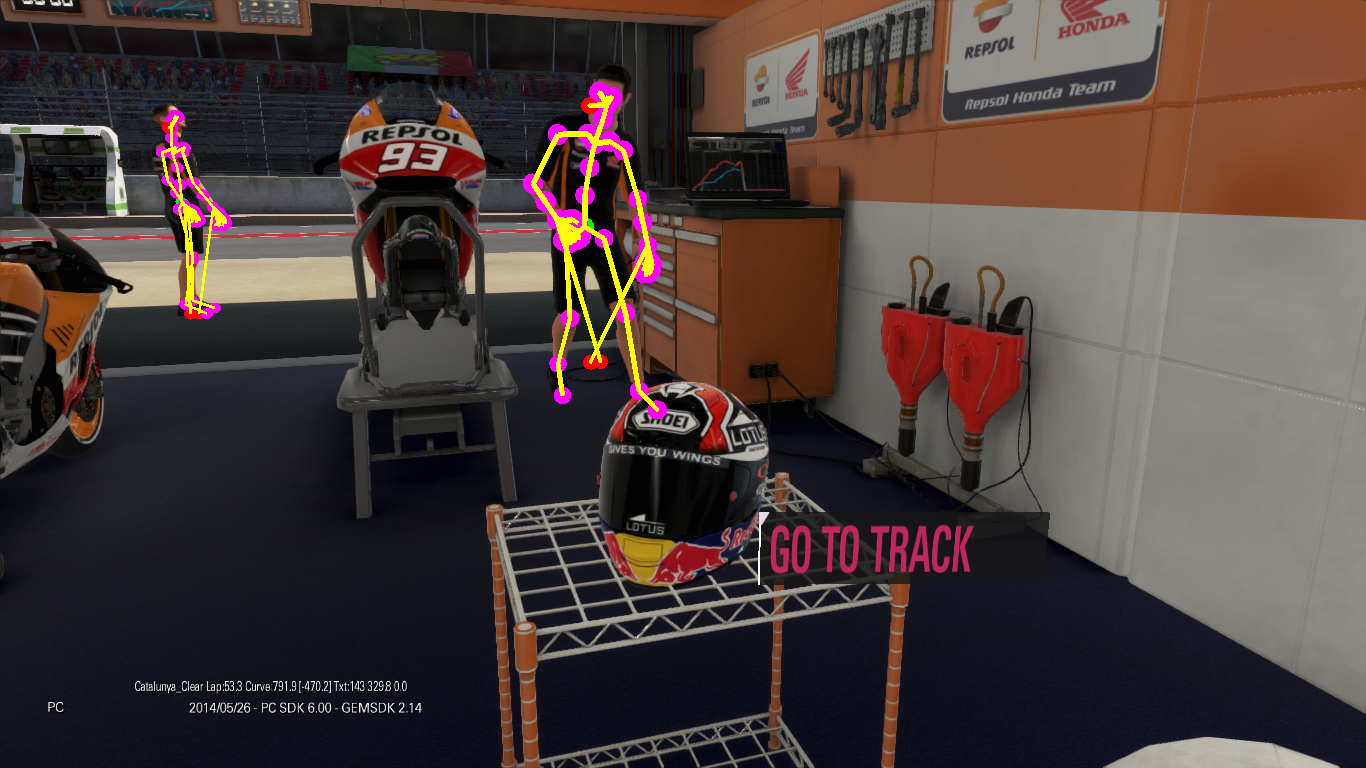
\includegraphics[width=1.1\columnwidth]{game/mechanicSkeleton.png} 
		\caption{Screenshot di MotoGP 14 in cui è stato attivato il disegno degli scheletri di animazione di 2 meccanici}
	\end{figure}
	
	Di seguito è presente il codice della classe \texttt{SkeletonDebugDrawerManager}.
	
	\lstinputlisting[style=maurizio-code, caption=SkeletonDebugDrawerManager.h, label={code:SkeletonDebugDrawerManager-h}]{code/SkeletonDebugDrawerManager.h}
	
	\lstinputlisting[style=maurizio-code, caption=SkeletonDebugDrawerManager.cpp, label={code:SkeletonDebugDrawerManager-cpp}]{code/SkeletonDebugDrawerManager.cpp}